\documentclass[conference]{IEEEtran}
\IEEEoverridecommandlockouts
% The preceding line is only needed to identify funding in the first footnote. If that is unneeded, please comment it out.
\usepackage{cite}
\usepackage{amsmath,amssymb,amsfonts}
\usepackage{algorithmic}
\usepackage{graphicx}
\usepackage{textcomp}
\usepackage{xcolor}
\def\BibTeX{{\rm B\kern-.05em{\sc i\kern-.025em b}\kern-.08em
    T\kern-.1667em\lower.7ex\hbox{E}\kern-.125emX}}
\begin{document}

\title{Fudge: An Agentic LLM-as-Judge for English-to-Filipino Translation of Western Animated Series\\
}

\author{\IEEEauthorblockN{John Kirsten Espiritu}
\IEEEauthorblockA{\textit{College of Computer Studies} \\
\textit{De La Salle University}\\
Manila, Philippines \\
john\_kirsten\_espiritu@dlsu.edu.ph}
\and
\IEEEauthorblockN{Elijah Nicolo Rosario}
\IEEEauthorblockA{\textit{College of Computer Studies} \\
\textit{De La Salle University}\\
Manila, Philippines \\
elijah\_rosario@dlsu.edu.ph}
}

\maketitle

\begin{abstract}
Summarize your project, methodology, and key findings, highlighting the comparison.
\end{abstract}

\begin{IEEEkeywords}
insert, keywords, here
\end{IEEEkeywords}

\section{Introduction}

The localization of media, such as television programs, into Filipino represents more than simple translation. It also serves as a way for cultural identity and language preservation to form in the Philippines. As documented by the \textit{National Commission for Culture and the Arts} (NCCA), early dependence on untranslated foreign programs from the early 1960s of Philippine television contributed to a \textit{colonial mentality} within Filipinos which can negatively affect both cultural and language development of the country \cite{correa_japanimation_2007,tuazon_philippine_nodate}. While Philippine television has overcome its preference for media in pure English as early as the conception of Filipino TV series in the early 1990s that are not just limited to entertainment, but also educational, such as \textit{Sine'skwela} and \textit{Math Tinik}, the importance of localizing foreign media into Filipino remains significant. 

\textit{Western Animated Series} (WAS) in particular have become a staple of Philippine television, with many series being broadcasted in localized Filipino, such as \textit{Avatar: The Last Airbender} or children's programs like \textit{Bob the Builder}. This is because the lack of localization for such series can create barriers to understanding for Filipino audiences of any age, or might even cause colonial mentality, the aforementioned preference for foreign media. This is particularly evident in the case of WAS, which often contain cultural references, humor, and language nuances that may not translate effectively into Filipino without careful adaptation. By effectively localizing these English animations, they not only become accessible to broader audiences but also become more relatable and culturally relevant to Filipino audiences, fostering a sense of national pride and cultural identity \cite{correa_japanimation_2007,marquez_halo-hallyung_2025}.

The process of localizing Western animated series for Philippine television presents unique challenges that extend beyond traditional translation work. Successful adaptation requires translation strategies that are accurate while also incorporating Filipino cultural elements \cite{marquez_halo-hallyung_2025}. However, achieving such quality consistently across the volume of content required for television broadcasting presents significant scalability challenges for human translators and localization teams.

Current methods employed by translation and localization teams to ensure quality of localization rely heavily on human expert evaluation. Human assessments and annotations by native speakers, though representing the gold standard in comprehensiveness through their holistic reasoning and cultural understanding, are costly, difficult to scale, and susceptible to inconsistency~\cite{gu_survey_2025}. Conversely, while automatic evaluation metrics such as BLEU~\cite{papineni_bleu_2001}, ROUGE~\cite{lin_rouge_2004}, chrF~\cite{popovic_chrf_2015}, and MatricX-24~\cite{juraska_metricx-24_2024} offer scalability and consistency, they can still fail to capture the deeper cultural and contextual nuances essential for effective localization, particularly in morphologically complex languages like Filipino where traditional n-gram metrics demonstrate poor performance~\cite{baliber_bridging_2020}.

To address these limitations, we propose leveraging \textit{LLM-as-a-Judge} as a complementary tool for translation and localization teams working on WAS. LLM-as-a-Judge systems have demonstrated the ability to merge the scalability of automatic methods with detailed, context-sensitive reasoning found in expert judgments~\cite{gu_survey_2025}, offering a promising solution to the persistent evaluation dilemma in translation quality assessment.

Furthermore, we evaluate the advantages of implementing \textit{agentic} LLM-as-a-Judge systems which are those equipped with external tool access, multi-step reasoning capabilities, and self-correction mechanisms, over traditional prompt-engineered approaches that rely solely on training data. Recent research demonstrates that tool-enabled LLMs can significantly outperform standard approaches, with agentic frameworks showing substantial improvements over few-shot prompting on complex tasks \cite{paranjape_art_2023}. For translation evaluation, agentic systems can access current cultural references, linguistic resources, and evaluation standards that pure training data cannot provide, while multistep reasoning enables sophisticated assessment processes that break down translation quality into supervised sub-tasks.

\section{Related Work}

Here, we discuss LLM-as-a-Judge systems, traditional evaluation methods, and the advantages of agentic systems over prompt-engineered approaches.

\subsection{Traditional Translation Metrics}

To contextualize the need for newer evaluation methods such as LLM-as-a-Judge, we must first understand the traditional metrics that have been used in Machine Translation (MT) evaluation. These metrics, while foundational, primarily operate on lexical and character-level comparisons, which have limitations when assessing translations for morphologically complex and culturally nuanced languages like Filipino.

\subsubsection{Bilingual Evaluation Understudy (BLEU)}

The \textit{Bilingual Evaluation Understudy} (BLEU) is a commonly used automatic MT evaluation, designed to measure the correspondence between a machine-generated translation and one or more high-quality human reference translations. It functions by calculating a modified n-gram precision score, comparing the co-occurrences of n-gram sequences in the candidate translation against the references \cite{papineni_bleu_2001}. While BLEU's speed and language independence have made it a widely adopted standard, its reliance on exact n-gram matching makes it less effective for languages with flexible word order and morphology, such as Filipino. For the creative and culturally-specific dialogue found in Western Animated Series, BLEU may fail to reward semantically correct but lexically divergent translations, thus providing an incomplete evaluation of localization quality \cite{juraska_metricx-24_2024}.

\subsubsection{Recall-Oriented Understudy for Gisting Evaluation (ROUGE)}

\textit{Recall-Oriented Understudy for Gisting Evaluation} (ROUGE) is a set of metrics originally developed for evaluating automatic text summarization. Unlike BLEU's precision focus, ROUGE is recall-oriented, measuring the number of n-grams from the human reference that are also found in the candidate text \cite{lin_rouge_2004}. This makes it effective at assessing whether the core information or "gist" of the source has been captured. In the context of translation, ROUGE can help determine if key phrases and concepts from the original dialogue are present in the Filipino localization. However, like BLEU, it is fundamentally a lexical overlap metric and struggles to evaluate semantic and cultural appropriateness beyond surface-level matches.

\subsubsection{Character n-gram F-score (chrF)}

The \textit{character n-gram F-score} (chrF) was proposed as an evaluation metric that operates at the character level, rather than the word level. The score is calculated as the F-score based on character n-gram precision and recall, with a variant, \textit{chrF3}, that gives three times more importance to recall. A key advantage of chrF is its independence from tokenization and its inherent ability to handle morphological variations, making it more suitable than word-based metrics for many languages \cite{popovic_chrf_2015}.

While chrF offers a more robust solution for morphologically complex languages like Filipino, its evaluation is still confined to surface-level text similarity. For the task of localizing animated series, which demands cultural resonance and the appropriate translation of idioms and humor, chrF cannot fully capture the quality of a translation that is lexically different but contextually superior \cite{montalan_batayan_2025}.

\subsubsection{MetricX-24}

More recent advancements in MT evaluation have moved towards learned metrics that aim to better correlate with human judgment. MetricX-24 is a state-of-the-art, regression-based metric built upon the mT5 language model. It operates as a hybrid reference-based and reference-free system, meaning it can score a translation with the source text, a reference text, or both. MetricX-24 is fine-tuned in two stages, first on \textit{Direct Assessment} (DA) ratings and then on a mixture of \textit{Multidimensional Quality Metrics} (MQM) and DA ratings. Its training is also augmented with synthetic data designed to improve robustness against common failure modes like undertranslation or fluent but unrelated outputs \cite{juraska_metricx-24_2024,montalan_batayan_2025}.

MetricX-24 represents an improvement over traditional lexical metrics by learning from human quality ratings. However, its output is a single quality score, which, while useful for benchmarking, provides limited actionable feedback for localization teams. Our work explores using an LLM-as-a-Judge not just for a quantitative score but for generating qualitative critiques that can directly guide translators in improving the cultural and contextual fit of WAS localizations.

\subsection{LLM-as-a-Judge}

The concept of \textit{LLM-as-a-Judge} has emerged as a powerful paradigm for automated evaluation, leveraging the advanced reasoning and language understanding capabilities of \textit{Large Language Models} (LLMs). This approach uses LLMs as evaluators for complex tasks, merging the scalability of automatic methods with the detailed, context-sensitive reasoning characteristic of human expert judgments. Formally, the process can be defined as $\mathcal{E} \leftarrow \mathcal{P}_{LLM}(x \oplus \mathcal{C})$, where an evaluation $\mathcal{E}$ is generated from an input $x$ combined with a context $\mathcal{C}$ (such as a prompt) by the LLM's probability function. This framework has been applied to a wide spectrum of evaluative roles, including graders, critics, and verifiers \cite{gu_survey_2025}.

Research shows that LLMs can serve as a compelling and cost-effective alternative to traditional human annotation, which is often slow and difficult to scale. LLM-as-a-Judge is particularly valuable for automating the annotation of large datasets and evaluating alignment with human preferences. This makes it a strong candidate for assessing the nuanced quality of translations where traditional metrics fall short.

Despite its potential, the reliability of LLM-as-a-Judge is a significant concern that requires careful system design and standardization. LLMs are susceptible to various biases, such as a preference for longer, more verbose responses (\textit{length bias)} or for answers appearing in a certain position within a prompt (\textit{position bias}). These biases can lead to inconsistent or unfair evaluations if not properly mitigated. The successful application of an LLM-as-a-Judge for a specialized domain like WAS localization is therefore highly dependent on its implementation. The following sections explore the two primary approaches to guiding LLM behavior for this task: direct prompt engineering and the creation of more autonomous, agentic systems.

\subsubsection{Prompt Engineering}

\textit{Prompt engineering} is the foundational method for guiding LLM behavior through \textit{In-Context Learning} (ICL), where task specifications, instructions, and examples are provided directly in the input prompt. The design of the prompt is critical, as it directly influences the model's ability to understand the task and generate a reliable evaluation. Best practices often involve \textit{few-shot prompting}, where several high-quality examples of the task are included in the prompt to help the LLM grasp the desired objectives and output format \cite{gu_survey_2025,sahoo_systematic_2025}.

To improve reliability and mitigate inherent model biases, prompt design strategies can include the decomposition of evaluation criteria into smaller, more explicit steps or shuffling the order of content to be compared to counteract position bias. Furthermore, constraining the model's output to a structured format, like JSON, and requiring it to provide explanations for its judgments can enhance both the robustness and the interpretability of the evaluation. However, prompts that are excessively long or complex can degrade performance, a phenomenon referred to as \textit{context rot}, making concise and clear instruction crucial \cite{hong_context_2025}. For our base model, we apply these principles to create a robust, prompt-engineered LLM-as-a-Judge, but this approach remains limited by the static information contained within the prompt itself.

\subsubsection{Agentic LLM Systems}

\textit{Agentic AI} represents an advancement from passive, instruction-following systems to autonomous agents capable of pursuing complex goals with minimal human supervision. Unlike traditional AI such as LLMs, which is often reactive, agentic systems are defined by their goal-oriented nature, adaptability, and capacity for strategic planning. A key distinction is their ability to leverage external tools and memory, enabling them to perform multi-step reasoning, retrieve real-time data from external sources like APIs, and learn from interactions with their environment \cite{kamoi_when_2024,hughes_ai_2025,acharya_agentic_2025}.

This capability to act voluntarily gives agentic systems a significant advantage over purely prompt-engineered models, which are usually limited to the knowledge learnt from training data and the context provided in the prompt. For a task like evaluating cultural localization, an agentic system can access up-to-date cultural references, consult online linguistic resources, or even query specialized translation databases to inform its judgment. This is particularly relevant for the dynamic and evolving nature of language and culture in the Philippines. Our study hypothesizes that an agentic LLM-as-a-Judge, through its ability to utilize external tools, will provide more accurate, current, and contextually-aware evaluations of English-to-Filipino WAS translations than its non-agentic counterpart.

\section{System Architecture}

Our LLM-as-a-Judge system for English-to-Filipino translation evaluation is designed around a core architectural principle of \\textit{dual-mode evaluation}, enabling comparative analysis between traditional prompt-engineered approaches and advanced agentic systems. The architecture follows a modular design that supports both evaluation paradigms while maintaining consistent input processing and output formatting, as illustrated in Figure~\\ref{fig:system_architecture}.

The system operates through a unified web application interface that processes translation evaluation requests through a standardized pipeline. Upon receiving user input consisting of the English source text, Filipino translation, and evaluation parameters, the system performs comprehensive input validation and preprocessing. This preprocessing phase includes token replacement for dynamic prompt construction and position randomization to mitigate the position bias commonly observed in LLM evaluations \\cite{gu_survey_2025}. The randomization mechanism shuffles the order of evaluation criteria presentation to ensure that judgments are based on content rather than positional preferences.

Central to our architecture is the implementation of two distinct evaluation modes: a \\textit{prompt-engineered judge} that relies exclusively on carefully crafted prompts and in-context learning, and an \\textit{agentic judge} (Fudge) that incorporates external tool access, multi-step reasoning, and autonomous planning capabilities. This dual-mode design enables direct comparison of evaluation approaches while maintaining architectural consistency in data flow and output structure.

Both evaluation modes operate on the same six-criteria assessment framework, evaluating translations based on accuracy, fluency, coherence, cultural appropriateness, guideline adherence, and completeness. Each criterion produces both a boolean judgment and detailed explanations, which are subsequently processed through a scoring algorithm that converts the boolean assessments into a standardized 1-5 scale rating. This structured output format ensures consistency across both evaluation modes and facilitates quantitative analysis of system performance.

The architecture incorporates robust error handling and logging mechanisms throughout the evaluation pipeline. All evaluation sessions are automatically stored with timestamped results, enabling comprehensive analysis of system behavior and consistency over time. The modular design also supports easy extension with additional LLM providers and evaluation criteria, making the system adaptable to evolving research needs and translation standards.

\begin{figure*}[htbp]
\centering
\includegraphics[width=\textwidth]{visuals/system-architecture.pdf}
\caption{System architecture of the LLM-as-a-Judge for English-to-Filipino translation of Western Animated Series.}
\label{fig:system_architecture}
\end{figure*}

\subsection{Prompt-Engineered Judge}

Describe its design (e.g., its comprehensive prompt, how it handles multi-turn inputs), emphasizing its lack of autonomous tool use and an explicit action-observation-reflection loop.

\subsubsection{Prompt Design}

Discuss your prompt engineering strategy for the pure judge.

\subsection{Agentic Judge (Fudge)}

\begin{figure}[htbp]
\centering
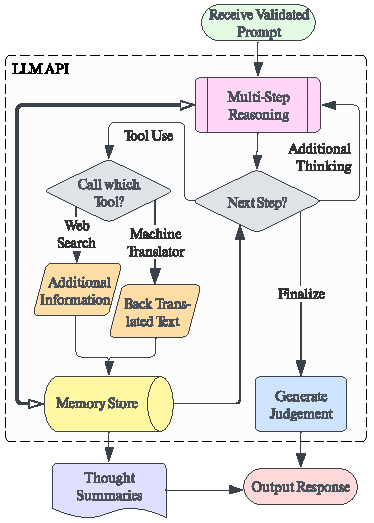
\includegraphics[width=\columnwidth]{fudge-architecture.pdf}
\caption{Architecture of the agentic judge (Fudge) showing the two-layer design with main agent orchestration and specialized sub-agents.}
\label{fig:fudge_architecture}
\end{figure}

The agentic judge, designated as Fudge, represents a significant departure from traditional prompt-engineered approaches through its implementation of autonomous tool usage, multi-step reasoning, and dynamic information retrieval. Fudge operates on a \textit{two-layer architecture} where the main agent, powered by Gemini 2.5 Pro or Flash, orchestrates the evaluation process while delegating specialized tasks to dedicated sub-agents. This design addresses the fundamental limitation of prompt-engineered systems that rely exclusively on training data and static context, enabling real-time access to current cultural references, linguistic resources, and translation standards essential for accurate localization assessment.

The system's orchestration mechanism allows the main agent to autonomously determine which tools are necessary for each specific translation case, rather than following a rigid evaluation sequence. When evaluating a translation containing cultural references or contemporary slang, for instance, Fudge may invoke multiple research queries through the search expert while simultaneously validating semantic preservation through back-translation analysis. This adaptive approach ensures that evaluation depth scales appropriately with translation complexity, providing thorough analysis for challenging cases while maintaining efficiency for straightforward translations.

Fudge's evaluation process follows a \textit{two-phase architecture}: an initial agentic generation phase that produces unstructured natural language assessment enriched with tool insights, followed by a structured conversion phase that transforms the analysis into the standardized six-criteria format. This design preserves the nuanced reasoning capabilities of the agentic system while ensuring compatibility with quantitative analysis requirements. The system captures comprehensive metadata throughout the process, including thought summaries that document the agent's reasoning process, function call logs that provide transparency into tool usage, and confidence indicators that reflect the system's assessment certainty.

\subsubsection{Available Tools}

\paragraph{Web Search Integration} The search expert tool provides Fudge with access to real-time information through a dedicated sub-agent equipped with Google Search capabilities. This tool addresses the critical limitation of static training data in evaluating contemporary cultural references, evolving language patterns, and current translation standards. When activated, the search expert creates a separate Gemini instance specifically configured for information retrieval, executing targeted searches based on the main agent's queries and returning contextualized results. For Western Animated Series localization, this capability proves essential when evaluating culturally-specific terminology, character names, or references that may have evolved since the model's training cutoff. The tool's integration follows a two-layer isolation design where search capabilities are separated from the main reasoning process, preventing conflicts between function calling mechanisms while ensuring comprehensive information access.

\paragraph{Machine Translation Validator} The back-translation validator serves as Fudge's primary semantic verification tool, implementing a round-trip translation methodology to assess meaning preservation. This tool translates the Filipino output back to English using Google Translate, then performs comparative analysis between the original source and back-translated text through word overlap calculations, length preservation ratios, and semantic similarity indicators. The validator provides quantitative metrics including word overlap ratios, common word identification, and semantic preservation quality ratings, enabling the main agent to make informed decisions about translation accuracy. This tool proves particularly valuable for detecting subtle semantic drift that may occur during cultural adaptation, ensuring that localization efforts enhance rather than compromise the original meaning.

\subsubsection{Prompt Design}

Discuss your prompt engineering strategy for the agentic judge.

\section{Methodology}

 Describe your dataset, experimental setup (which LLM, frameworks), and how you'll evaluate both judges using metrics like consistency, alignment with human judgment, and explainability.

 
\section{Results and Discussion}


Comparative Analysis: Present quantitative results for both judges side-by-side.

Qualitative Comparison: Show examples of evaluations from both judges, discussing their strengths, weaknesses, and reasoning.

Discussion of Differences: Analyze why one approach might perform better, highlighting the impact of your agent's design choices (e.g., tools, planning) versus the prompt-engineered approach. Discuss insights in light of the Gu et al. (2025) paper.


\section{Conclusion and Future Work}

Summarize your findings, emphasizing the insights from your comparison. Discuss limitations of your designs and suggest future improvements.

\section*{Figures and Tables}
\paragraph{Positioning Figures and Tables} Place figures and tables at the top and 
bottom of columns. Avoid placing them in the middle of columns. Large 
figures and tables may span across both columns. Figure captions should be 
below the figures; table heads should appear above the tables. Insert 
figures and tables after they are cited in the text. Use the abbreviation 
``Fig.~\ref{fig}'', even at the beginning of a sentence.

\begin{table}[htbp]
\caption{Table Type Styles}
\begin{center}
\begin{tabular}{|c|c|c|c|}
\hline
\textbf{Table}&\multicolumn{3}{|c|}{\textbf{Table Column Head}} \\
\cline{2-4} 
\textbf{Head} & \textbf{\textit{Table column subhead}}& \textbf{\textit{Subhead}}& \textbf{\textit{Subhead}} \\
\hline
copy& More table copy$^{\mathrm{a}}$& &  \\
\hline
\multicolumn{4}{l}{$^{\mathrm{a}}$Sample of a Table footnote.}
\end{tabular}
\label{tab1}
\end{center}
\end{table}

\begin{figure}[htbp]
\centerline{\includegraphics{fig1.png}}
\caption{Example of a figure caption.}
\label{fig}
\end{figure}

Figure Labels: Use 8 point Times New Roman for Figure labels. Use words 
rather than symbols or abbreviations when writing Figure axis labels to 
avoid confusing the reader. As an example, write the quantity 
``Magnetization'', or ``Magnetization, M'', not just ``M''. If including 
units in the label, present them within parentheses. Do not label axes only 
with units. In the example, write ``Magnetization (A/m)'' or ``Magnetization 
\{A[m(1)]\}'', not just ``A/m''. Do not label axes with a ratio of 
quantities and units. For example, write ``Temperature (K)'', not 
``Temperature/K''.

\bibliographystyle{ieeetr}
% \nocite{*}
\bibliography{llm_references}  

\end{document}
